In this section, we go through a first example dealing with the Poisson equation. At first we introduce the mathematical setting and well-posedness of the problem, presenting its finite dimensional formulation and the error estimates. Then we explain how to solve the Poisson problem using LifeV, going through the different stages that characterize the simulation. More in particular, we will cover the following topics: 
\begin{itemize}
	\item the preamble: including the headers and configuring MPI
	\item the construction of a structured mesh and the definition of the finite elements space
	\item the assembly of the stiffness matrix, the right-hand-side and the setting of boundary conditions
	\item the preconditioner and the solution of the linear system
	\item the exporting of data and the post-processing
\end{itemize}



\subsection{Variational formulation and finite element discretization}
Let $ \Omega \subset \mathbb{R}^d, \, d = 2,3 $ be a regular open bounded domain and let $  \partial \Omega $ be its boundary such that $ \partial \Omega = \Gamma_D \cup \Gamma_N$, $ \mathring{\Gamma}_D \cap \mathring{\Gamma}_N = \emptyset $, our problem reads

\begin{align}
\begin{cases}
\nonumber
-\Delta u = f \qquad & \mathbf{x} \in \Omega,
\\  \label{eq:poisson}
u = g(\mathbf{\sigma}) \qquad & \mathbf{\sigma} \in \Gamma_D,
\\ \nonumber
\partial_n u = h(\mathbf{\sigma}) \qquad & \mathbf{\sigma} \in \Gamma_N,
\end{cases}
\end{align}
\noindent
where $ f = f(\mathbf{x}) $ denotes the source term and $  g(\mathbf{\sigma}), h(\mathbf{\sigma}) $ denote the Dirichlet and Neumann boundary conditions, respectively. Starting from the differential equation, we can derive the weak formulation of the problem. We introduce the spaces
\begin{align}
	V &= H^1_d(\Omega) = \Bigl\{ v \in H^1(\Omega): v|_{\Gamma_D} = 0 \Bigr\}
\end{align}
and
\begin{align}
	V_g &= \Bigl\{ v \in H^1(\Omega): v|_{\Gamma_D} = g(\sigma) \Bigr\}.
\end{align}
Finally, our problem reads: find $ u \in V_g $, such that  
\begin{align}\label{eq:varPoisson}
a(u, v) = Fv \qquad \forall v \in V,
\end{align}
where
\begin{align} 
	a(u, v) = \int_{\Omega} \nabla u \cdot \nabla v d\mathbf{x} \qquad 
	\text{ and } \qquad 
	Fv = \int_{\Omega} f(\mathbf{x}) d\mathbf{x} + \int_{\Gamma_N} h(\sigma) d\sigma.
\end{align}
Under appropriate hypothesis, problem \eqref{eq:varPoisson} is well-posed.
In order to obtain a discrete solution of problem \eqref{eq:varPoisson} based on the finite element method, we introduce at first a partition $ \mathcal{T}_h $ of the domain $ \Omega $, and the finite-dimensional space
\begin{align}
V_h = X_h^r = \Bigl\{ v_h \in C^0(\bar{\Omega}): v_h|_K \in \mathbb{P}^r(), \forall K \in \mathcal{T}_h \Bigr\},
\end{align}
where $ \mathbb{P}^r $ denotes the polynomial functions of degree lower than or equal to $ r $. For sake of simplicity we suppose homogeneous Dirichlet boundary conditions, i.e. $ g = 0 $, in case $ g \neq 0 $, it is possible to operate a lifting to ring back to the homogeneous case. 
\newline \noindent
Finally, the finite dimensional problem reads: find $ u_h \in V_h $ such that 
\begin{align}\label{eq:fePoisson}
a(u_h, v_h) = Fv_h \qquad v_h \in V_h.
\end{align}
Starting from equation \eqref{eq:fePoisson}, it is possible to write the problems in the form of a linear system, and it is possible to prove that under appropriate assumptions about the data and the regularity of the exact solution $ u $, the discrete solution $ u_h $ satisfies the following error estimates
\begin{align}\label{eq:stimaHL}
& \|u-u_h\|_{L^2(\Omega)}  \leq Ch^{r+1}|u|_{H^{r+1}}, \\ &\nonumber \\ \label{eq:stimaH1}
& \|u-u_h\|_{H^1(\Omega)}  \leq Ch^r|u|_{H^{r+1}},
\end{align}
where $ h $ denotes the characteristic size of the mesh, $r$ the polynomial degree employed and $ C $ is a constant independent of $ h $ and $ u $, see e.g. \cite{CMCSBOOK2009002}.

\subsection{LifeV simulation}
To the aim of solving problem \eqref{eq:fePoisson} using LifeV, we set $ \Omega = (-1, 1)^3 $, $ \Gamma_D = \partial \Omega $ and the data $f, \, g, \, h $ such that the exact solution of the Poisson problem is  $ u(\mathbf{x}) = sin(\pi x)sin(\pi y)sin(\pi z) $.
\subsubsection*{Preamble: headers and MPI configuration}
We first include the different headers containing the data structures and the algorithms we are employing along the simulation: At first the Epetra data structures that allow the use of MPI
\begin{itemize}
\item the definition of the MPI environment, that is made exploiting the Epetra framework
\begin{lstlisting}
#include <Epetra_ConfigDefs.h>
#ifdef EPETRA_MPI
#include <mpi.h>
#include <Epetra_MpiComm.h>
#else
#include <Epetra_SerialComm.h>
#endif
\end{lstlisting}
\item the definition of the basis structures of LifeV, in particular meshes, finite elements spaces and expressions
\begin{lstlisting}
#include <lifev/core/LifeV.hpp>
#include <lifev/core/util/LifeChronoManager.hpp>
#include <lifev/core/mesh/MeshPartitioner.hpp>
#include <lifev/core/mesh/RegionMesh3DStructured.hpp>
#include <lifev/core/mesh/RegionMesh.hpp>
#include <lifev/core/array/MatrixEpetra.hpp>
#include <lifev/core/fem/BCManage.hpp>
#include <lifev/eta/fem/ETFESpace.hpp>
#include <lifev/eta/expression/BuildGraph.hpp>
#include <lifev/eta/expression/Integrate.hpp>
#include <Epetra_FECrsGraph.h>
\end{lstlisting}
\item the definition of the solver and the exporting routines
\begin{lstlisting}
#include <Teuchos_ParameterList.hpp>
#include <Teuchos_XMLParameterListHelpers.hpp>
#include <Teuchos_RCP.hpp>
#include <lifev/core/algorithm/LinearSolver.hpp>
#include <lifev/core/algorithm/PreconditionerIfpack.hpp>
#include <lifev/core/filter/ExporterHDF5.hpp>
\end{lstlisting}
\item some other useful classes
\begin{lstlisting}
#include <boost/shared_ptr.hpp>
#include <lifev/eta/examples/laplacian/laplacianFunctor.hpp>
\end{lstlisting}
Next, we define the LifeV namespace

\begin{lstlisting}
using namespace LifeV;


\end{lstlisting}

\subsubsection*{Structured mesh and finite element spaces}
After having read the datafile as explained in Section \ref{sec:readingData}, we build a cubic structured mesh and we divide it among the processors which are running the simulation

\begin{lstlisting}
// Mesh
typedef RegionMesh< LinearTetra > mesh_Type;
std::shared_ptr< mesh_Type > fullMeshPtr ( new mesh_Type ( Comm ) );
 
// Building structured mesh (in this case a cube)
regularMesh3D ( *fullMeshPtr, 0,
        dataFile( "mesh/nx", 15 ), dataFile( "mesh/ny", 15 ), 
        dataFile( "mesh/nz", 15 ), dataFile ( "mesh/verbose", false ),
        2.0, 2.0, 2.0, -1.0,-1.0, -1.0 );

// Partitioning mesh, possibly with overlap
const UInt overlap ( dataFile( "mesh/overlap", 0 ) );
std::shared_ptr< mesh_Type > localMeshPtr;

MeshPartitioner< mesh_Type > meshPart;

if ( overlap )
{
    meshPart.setPartitionOverlap ( overlap );
}
   
meshPart.doPartition ( fullMeshPtr, Comm );
localMeshPtr = meshPart.meshPartition();

// Clearing global mesh
fullMeshPtr.reset();
\end{lstlisting}    
We notice that the domain origins from the point $ (-1 -1, -1) $ and has a length of 2 in each dimension. The \verb!overlap! variable states the number of layers that are shared by two processors with contiguous subdomains.
\newline \noindent
We next define the finite element space, whose dimension is read by the input file. Then we build the corresponding Expression Template finite element space, whose use allows the user to adopt the templated expressions that refer to the weak formulation of the problem.
\begin{lstlisting}
// Finite element space
typedef FESpace< mesh_Type, MapEpetra >                 uSpaceStd_Type;
typedef std::shared_ptr< uSpaceStd_Type >             uSpaceStdPtr_Type;
typedef ETFESpace< mesh_Type, MapEpetra, 3, 1 >         uSpaceETA_Type;
typedef std::shared_ptr< uSpaceETA_Type >             uSpaceETAPtr_Type;
typedef FESpace<mesh_Type, MapEpetra>::function_Type    function_Type;

// Defining finite elements standard and Expression Template spaces
uSpaceStdPtr_Type uFESpace ( new uSpaceStd_Type ( localMeshPtr, 
                    dataFile( "finite_element/degree", "P1" ), 1, Comm ) );
uSpaceETAPtr_Type ETuFESpace ( new uSpaceETA_Type ( localMeshPtr, 
                    & ( uFESpace->refFE() ), & ( uFESpace->fe().geoMap() ), Comm ) );
\end{lstlisting}  

\subsubsection*{Assembly of the stiffness matrix, the right-hand-side and the setting of boundary conditions}
In order to assembly the system that corresponds to the finite element formulation, we need to build at first the graph that contains the topology of the matrix and then assemblying the matrix by constructing the elements $ a(\phi_j,\phi_i) $
\begin{lstlisting}
// Matrices and graphs
typedef Epetra_FECrsGraph                               graph_Type;
typedef std::shared_ptr<Epetra_FECrsGraph>            graphPtr_Type;
typedef MatrixEpetra< Real >                            matrix_Type;
typedef std::shared_ptr< MatrixEpetra< Real > >       matrixPtr_Type;

graphPtr_Type systemGraph;
matrixPtr_Type systemMatrix;

if ( overlap )
{
    systemGraph.reset ( new graph_Type ( Copy, * ( uFESpace->map().map( Unique ) ), 50, true ) );
}
else
{
    systemGraph.reset ( new graph_Type ( Copy, * ( uFESpace->map().map( Unique ) ), 50 ) );
}

{
    using namespace ExpressionAssembly;
    
    buildGraph (
            elements ( localMeshPtr ),
            uFESpace->qr(),
            ETuFESpace,
            ETuFESpace,
            dot ( grad ( phi_i ) , grad ( phi_j ) )
        )
        >> systemGraph;
}

systemGraph->GlobalAssemble();

if ( overlap )
{
systemMatrix.reset( new matrix_Type ( ETuFESpace->map(), *systemGraph, true ) );
}
else
{
systemMatrix.reset( new matrix_Type ( ETuFESpace->map(), *systemGraph ) );
}

// Clearing problem's matrix
systemMatrix->zero();

{
    using namespace ExpressionAssembly;
    
    integrate (
            elements ( localMeshPtr ),
            uFESpace->qr(),
            ETuFESpace,
            ETuFESpace,
            dot ( grad ( phi_i ) , grad ( phi_j ) )
        )
        >> systemMatrix;
}
\end{lstlisting}
Next, we build the solution and the right hand side vectors. For the latter, we employ the \verb!laplacianFunctor! class, that is constructed by providing the function that describes the source term
\begin{lstlisting}
// Vectors
typedef VectorEpetra                                    vector_Type;
typedef std::shared_ptr<VectorEpetra>                 vectorPtr_Type;

vectorPtr_Type rhsLap;
vectorPtr_Type solutionLap;

if ( overlap )
{
    rhsLap.reset ( new vector_Type ( uFESpace->map(), Unique, Zero ) );
    solutionLap.reset ( new vector_Type ( uFESpace->map(), Unique, Zero ) );
}
else
{
    rhsLap.reset ( new vector_Type ( uFESpace->map(), Unique ) );
    solutionLap.reset ( new vector_Type ( uFESpace->map(), Unique ) );
}

rhsLap->zero();
solutionLap->zero();

Real sourceFunction ( const Real& /*t*/, const Real& x, 
                      const Real& y, const Real& z, 
                      const ID& /*i*/)
{
    return 3 * M_PI * M_PI 
             * sin( M_PI * x )  * sin( M_PI * y ) * sin( M_PI * z );
}

std::shared_ptr<laplacianFunctor< Real > >  laplacianSourceFunctor ( new laplacianFunctor< Real >( sourceFunction ) );

{
    using namespace ExpressionAssembly;
    
    integrate (
            elements ( localMeshPtr ),
            uFESpace->qr(),
            ETuFESpace,
            eval(laplacianSourceFunctor, X) * phi_i
        )
        >> rhsLap;
}
\end{lstlisting}
We remark here that the use of the expression templates allows the user to define the equivalent of the weak formulation, in particular the elements of the matrix are built using the test and trial functions $ phi_i $ and $ phi_j $, and setting the quadrature rule to adopt.

\subsubsection*{Boundary conditions}
We explain here how to impose the boundary conditions. At first we give an identification number to the faces of our domain, and then define the function $ g $ that is assigned to the boundarues, in this case we have homogeneous Dirichlet conditions, so we construct the function \verb!zeroFunction! that returns 0. for every value of the spatial domain. In LifeV, it is possible to impose the boundaries through a BCHandler object, which imposes on every boundary the corresponding Dirichlet datum by providing the keyword \verb!Essential!.
\begin{lstlisting}
// Cube's walls identifiers
const int BACK   = 1;
const int FRONT  = 2;
const int LEFT   = 3;
const int RIGHT  = 4;
const int BOTTOM = 5;
const int TOP    = 6;

Real zeroFunction (const Real& /*t*/, const Real& /*x*/, const Real& /*y*/, const Real& /*z*/, const ID& /*i*/)
{
    return 0.;
}

BCHandler bcHandler;

BCFunctionBase ZeroBC ( zeroFunction );
BCFunctionBase OneBC ( nonZeroFunction );

bcHandler.addBC( "Back",   BACK,   Essential, Scalar, ZeroBC, 1 );
bcHandler.addBC( "Left",   LEFT,   Essential, Scalar, ZeroBC, 1 );
bcHandler.addBC( "Top",    TOP,    Essential, Scalar, ZeroBC, 1 );
bcHandler.addBC( "Front",  FRONT,  Essential, Scalar, ZeroBC, 1 );
bcHandler.addBC( "Right",  RIGHT,  Essential, Scalar, ZeroBC, 1 );
bcHandler.addBC( "Bottom", BOTTOM, Essential, Scalar, ZeroBC, 1 );

bcHandler.bcUpdate( *uFESpace->mesh(), uFESpace->feBd(), uFESpace->dof() );
bcManage ( *systemMatrix, *rhsLap, *uFESpace->mesh(), uFESpace->dof(), 
            bcHandler, uFESpace->feBd(), 1.0, 0.0 );
\end{lstlisting}

\subsubsection*{Preconditioning and solving the system}
Since our computation employs a parallel architecture. before solving the linear system we need to assemble both the matrix and the right hand side
\begin{lstlisting}
systemMatrix->globalAssemble();
rhsLap->globalAssemble();
\end{lstlisting}
Next we set the solver parameters according to the input file \verb!SolverParamList.xml! and the preconditioner that employs the Additive Schwarz method
\begin{lstlisting}
// Solver and preconditioner
typedef LinearSolver::SolverType                        solver_Type;
typedef LifeV::Preconditioner                           basePrec_Type;
typedef std::shared_ptr<basePrec_Type>                basePrecPtr_Type;
typedef PreconditionerIfpack                            prec_Type;
typedef std::shared_ptr<prec_Type>                    precPtr_Type;

LinearSolver linearSolver ( Comm );
linearSolver.setOperator ( systemMatrix );

Teuchos::RCP< Teuchos::ParameterList > aztecList = Teuchos::rcp ( new Teuchos::ParameterList );
aztecList = Teuchos::getParametersFromXmlFile ( "SolverParamList.xml" );

linearSolver.setParameters ( *aztecList );

prec_Type* precRawPtr;
basePrecPtr_Type precPtr;
precRawPtr = new prec_Type;
precRawPtr->setDataFromGetPot ( dataFile, "prec" );
precPtr.reset ( precRawPtr );

linearSolver.setPreconditioner ( precPtr );
\end{lstlisting}
And finally we solve the system
\begin{lstlisting}
linearSolver.setRightHandSide( rhsLap );
linearSolver.solve( solutionLap );
\end{lstlisting}



\subsubsection*{Exporting and post processing}
We set the exporter that employs the library HDF5, the result is then visible using a post processing tool, for instance Paraview (\url{http://www.paraview.org/}).
\begin{lstlisting}
// Setting exporter
ExporterHDF5< mesh_Type > exporter ( dataFile, "exporter" );
exporter.setMeshProcId( localMeshPtr, Comm->MyPID() );
exporter.setPrefix( "laplace" );
exporter.setPostDir( "./" );
exporter.addVariable ( ExporterData< mesh_Type >::ScalarField, "temperature", uFESpace, solutionLap, UInt ( 0 ) );
exporter.postProcess( 0 );
exporter.closeFile();
\end{lstlisting}

\begin{figure}
    \centering
    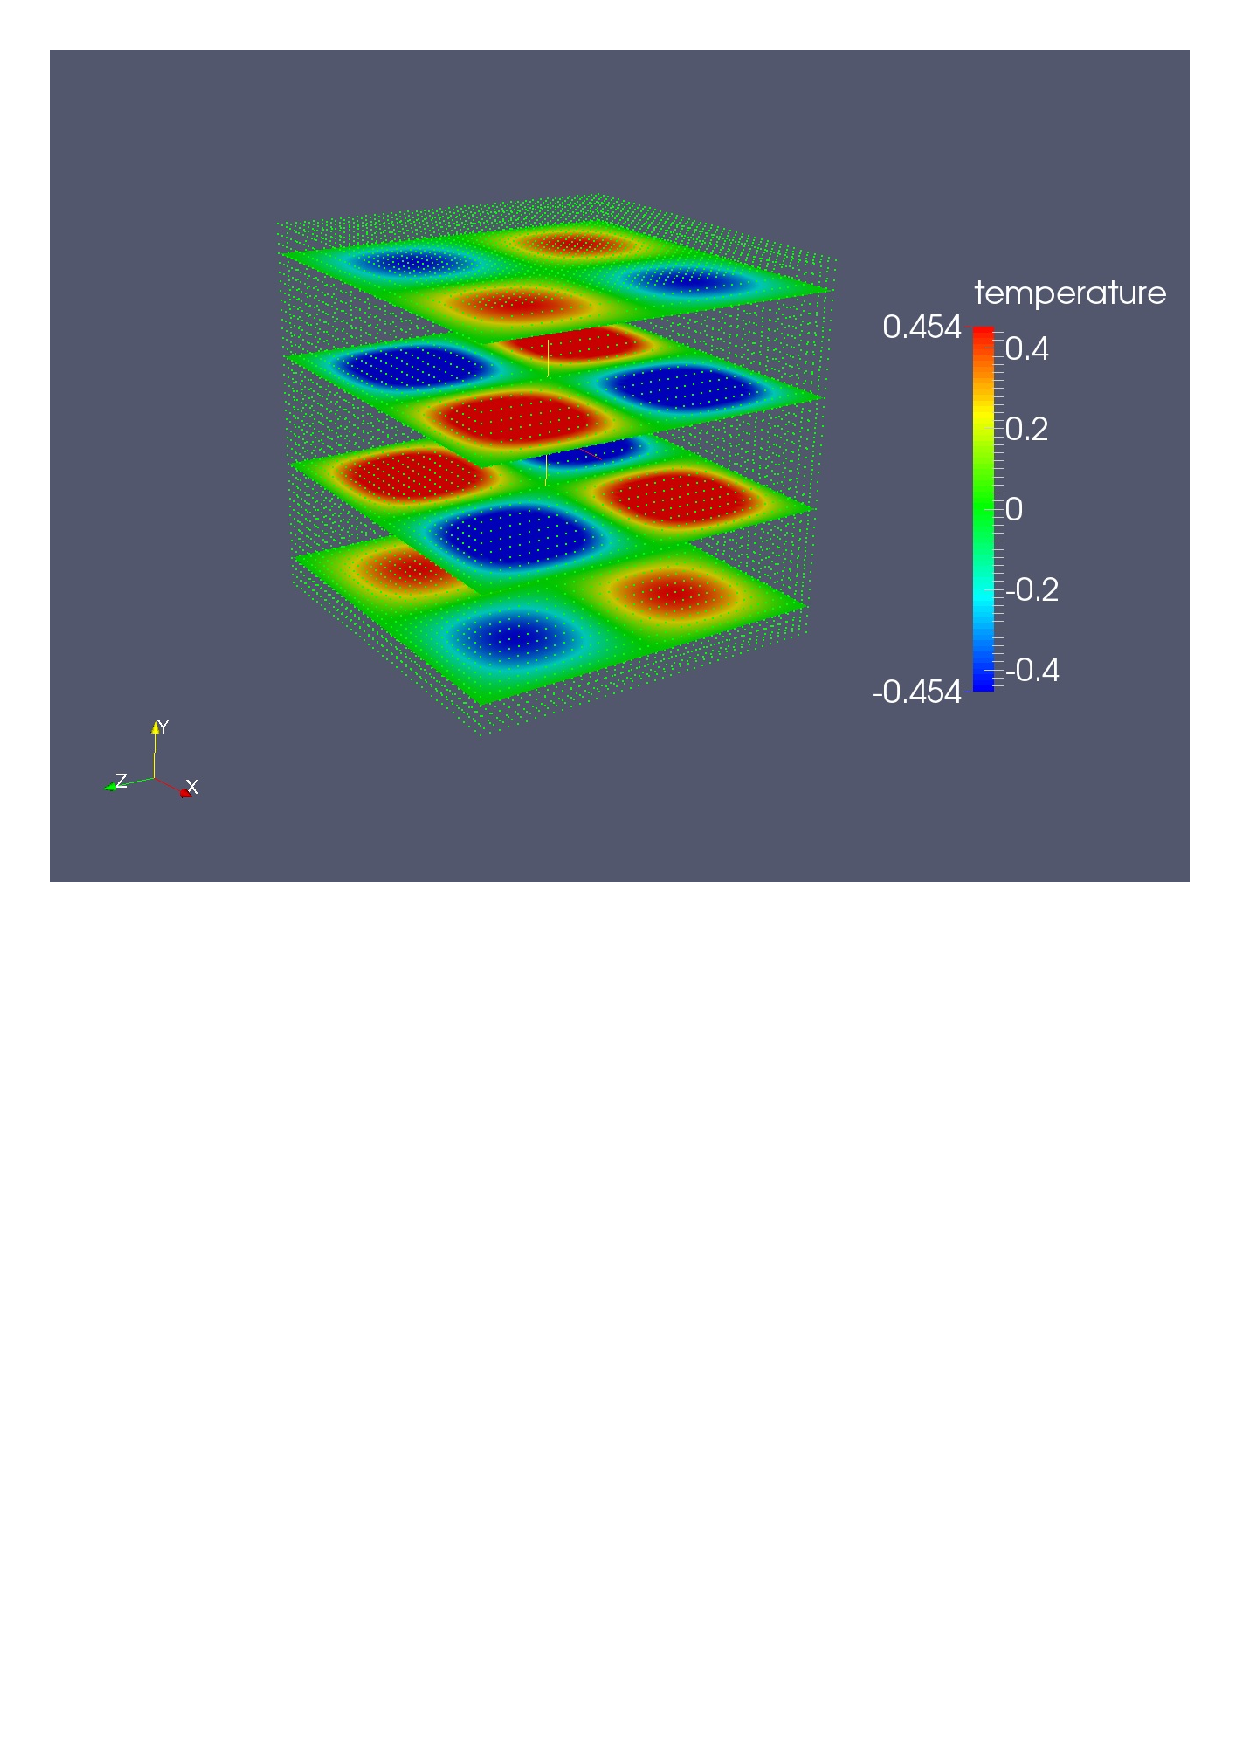
\includegraphics[width=\linewidth, trim=0cm 15cm 0cm 0cm, clip=true ]{pictures/slices}
    \caption{Result of Poisson equation with homogeneous Dirichlet boundary conditions}
    \label{fig:lap1}
\end{figure}
 
\newline \noindent
Now, suppose we want to investigate the trend of the error by varying the mesh size, to check numerically the estimates \eqref{eq:stimaHL}, \eqref{eq:stimaH1}. At first, we need to define the function $ u $ and its gradient $ \nabla u $ in our program, in the same way we defined the source term $f$
\begin{lstlisting}
Real uExactFunction (const Real& /*t*/, const Real& x, const Real& y, const Real& z, const ID& /*i*/)
{
    return sin( M_PI * y ) * sin( M_PI * z ) * sin ( M_PI * x );
}

function_Type uEx(uExactFunction);

VectorSmall< 3 > uGradExactFunction (const Real& /*t*/, const Real& x, const Real& y, const Real& z, const ID& /*i*/)
{
    VectorSmall< 3 > v;
    
    v[0] = M_PI * cos( M_PI * x ) * sin( M_PI * y ) * sin( M_PI * z );
    v[1] = M_PI * sin( M_PI * x ) * cos( M_PI * y ) * sin( M_PI * z );
    v[2] = M_PI * sin( M_PI * x ) * sin( M_PI * y ) * cos( M_PI * z );
    
    return v;
}

std::shared_ptr<laplacianFunctor< Real > >  laplacianExactFunctor ( new laplacianFunctor< Real >( uExactFunction ) );
std::shared_ptr<laplacianFunctor< VectorSmall<3> > >  laplacianExactGradientFunctor ( new laplacianFunctor< VectorSmall<3> >( uGradExactFunction ) );
\end{lstlisting}
Next, we need to evaluate the norms following their definition, and to do that we still employ the Expression Templates provided in LifeV
\begin{lstlisting}
Real L2ErrorLap = 0.0;
Real TotL2ErrorLap = 0.0;

Real H1SeminormLap = 0.0;
Real TotH1SeminormLap = 0.0;

{
    using namespace ExpressionAssembly;

    integrate (
            elements ( localMeshPtr ),
            uFESpace->qr(),
            ( eval(laplacianExactFunctor, X) - value (ETuFESpace, *solutionLap) )
            * ( eval(laplacianExactFunctor, X) - value (ETuFESpace, *solutionLap) )
        ) >> L2ErrorLap;

}

{
    using namespace ExpressionAssembly;
    
    integrate (
            elements ( localMeshPtr ),
            uFESpace->qr(),
            dot( eval(laplacianExactGradientFunctor, X) - grad( ETuFESpace, *solutionLap ),
            eval(laplacianExactGradientFunctor, X) - grad( ETuFESpace, *solutionLap ) )
        ) >> H1SeminormLap;
 
}
Comm->Barrier();
\end{lstlisting}
Finally, we gather the results of the different processors and print the norm. We collect the results for different mesh sizes and perform a convergence analysis, whose results are shown in Fig. \ref{fig:normHL}.
\begin{lstlisting}
Comm->SumAll (&L2ErrorLap, &TotL2ErrorLap, 1);
Comm->SumAll (&H1SeminormLap, &TotH1SeminormLap, 1);

if (verbose)
{
    std::cout << "TotError in L2 norm is " 
              << sqrt( TotL2ErrorLap ) << std::endl;
    std::cout << "TotError in H1 norm is " 
              << sqrt( TotL2ErrorLap + TotH1SeminormLap ) << std::endl;    
}
\end{lstlisting}

 
\begin{figure}
    \subfloat{
            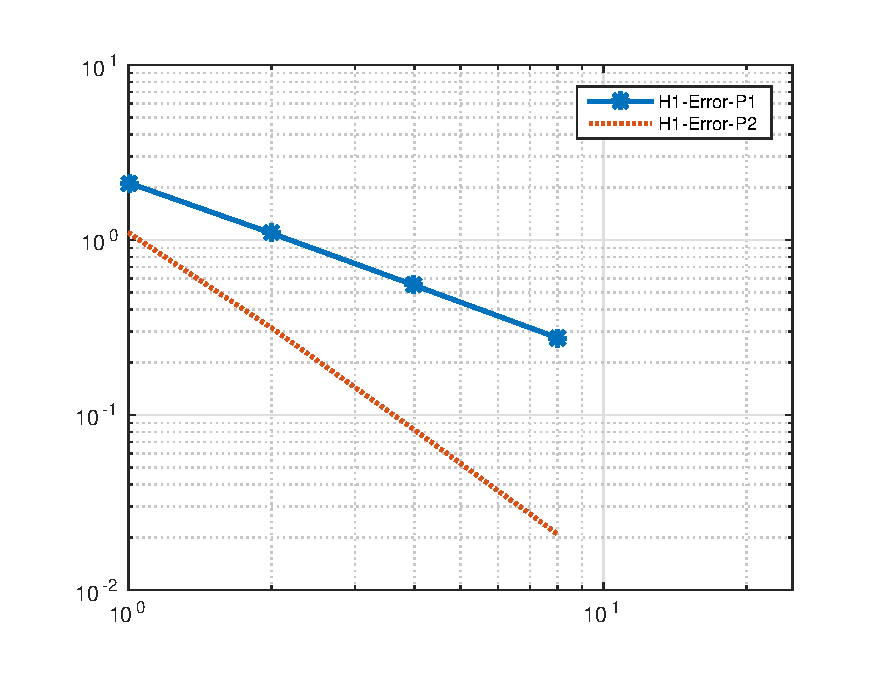
\includegraphics[width=.45\textwidth ]{pictures/convH1}
            }
    \subfloat{
            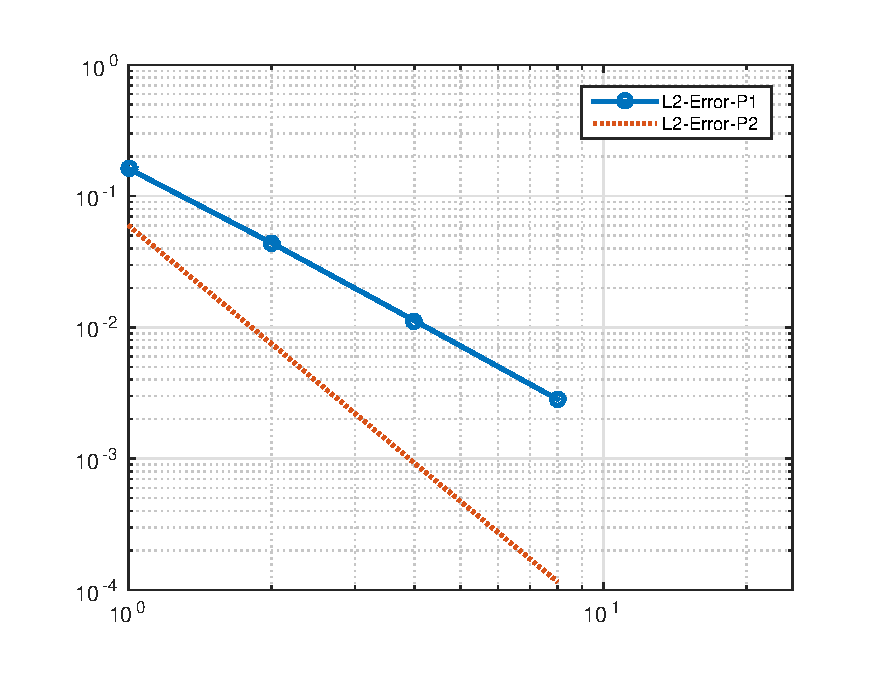
\includegraphics[width=.45\textwidth ]{pictures/convL2}
            }
    \caption{$H^1$ norm (left) and $L^2$ norm (right) vs mesh size for $ r =1,\, 2$.}
    \label{fig:normHL}
\end{figure}

